
\chapter{Sorting}
\section{Bubble Sort}
Bubble sort is a fairly simple sorting algorithm and involves comparing 2 adjacent list items and swapping them if they are not in order. Bubble sort is implemented with 2 nested loops, so that for each of the "iterations" (one full loop) the next highest number is properly placed. \newline

It is not ideal for large data sets since its worst case complexity is O(n\textsuperscript{2}).\newline

Note: bubble sort can also be implemented by starting index n, and placing the next smallest value in each iteration

\begin{figure}[H]
\centering
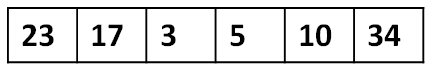
\includegraphics[width=0.3\textwidth]{pictures/bubble1.png}
\caption{Unsorted Data Set}
\label{fig:bubble1}
\end{figure}

\begin{figure}[H]
\centering
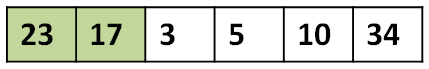
\includegraphics[width=0.3\textwidth]{pictures/bubble2.png}
\label{fig:bubble2}
\end{figure}

1\textsuperscript{st} iteration, index 5 should be correct at the end.
Comparing 23 and 17, a switch is needed.

\begin{figure}[H]
\centering
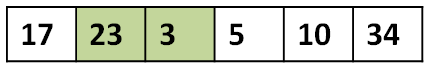
\includegraphics[width=0.3\textwidth]{pictures/bubble3.png}
\label{fig:bubble3}
\end{figure}

23 and 17 switched. Comparing 23 and 3, a switch is needed.

\begin{figure}[H]
\centering
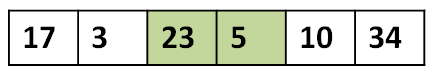
\includegraphics[width=0.3\textwidth]{pictures/bubble4.png}
\label{fig:bubble4}
\end{figure}

23 and 3 are switched. Comparing 23 and 5, a switch is needed.

\begin{figure}[H]
\centering
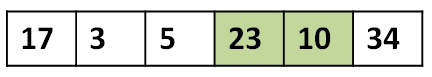
\includegraphics[width=0.3\textwidth]{pictures/bubble5.png}
\label{fig:bubble5}
\end{figure}

23 and 5 switched. Comparing 23 and 10, a switch is needed.

\begin{figure}[H]
\centering
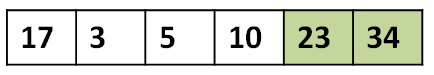
\includegraphics[width=0.3\textwidth]{pictures/bubble6.png}
\label{fig:bubble6}
\end{figure}

23 and 10 switched. Comparing 23 and 34, no switch needed. 

\begin{figure}[H]
\centering
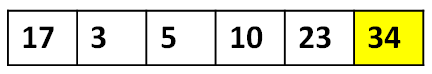
\includegraphics[width=0.3\textwidth]{pictures/bubble7.png}
\label{fig:bubble7}
\end{figure}

End of data set, 34 is in the correct place.

\begin{figure}[H]
\centering
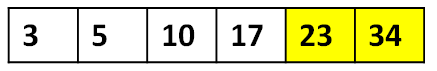
\includegraphics[width=0.3\textwidth]{pictures/bubble8.png}
\label{fig:bubble8}
\end{figure}

End of 2\textsuperscript{nd} iteration, 23 is placed correctly.

*Note: The lower indexed places have been sorted a second time.

\begin{figure}[H]
\centering
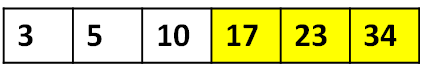
\includegraphics[width=0.3\textwidth]{pictures/bubble9.png}
\label{fig:bubble9}
\end{figure}

End of 3\textsuperscript{rd} iteration, 17 is placed correctly.

*Note: The lower indexed places have been sorted a third time even its order was already correct.

\begin{figure}[H]
\centering
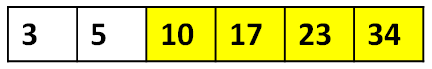
\includegraphics[width=0.3\textwidth]{pictures/bubble10.png}
\label{fig:bubble10}
\end{figure}

End of 4\textsuperscript{th} iteration, 10 is placed correctly.

\begin{figure}[H]
\centering
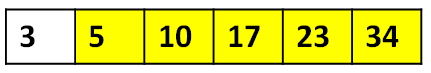
\includegraphics[width=0.3\textwidth]{pictures/bubble11.png}
\label{fig:bubble11}
\end{figure}

End of 5\textsuperscript{th} iteration, 5 is placed correctly.

\begin{figure}[H]
\centering
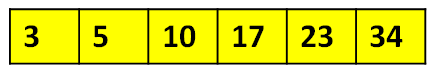
\includegraphics[width=0.3\textwidth]{pictures/bubble12.png}
\label{fig:bubble12}
\end{figure}

3 is placed correctly. No iteration should be needed for index 0, since the smallest value would have been placed correctly from the previous iteration.

\subsection{Pseudocode}

\begin{verbatim}
bubbleSort(List):List
            for(iteration: all elements in the list)
                for(i: from 0 to iteration)
                    if List[i] > List[i+1]
                        swap(List[i], List[i+1])
            return List
\end{verbatim}

\section{Selection Sort}
Selection sort works by finding the smallest item in the data set and placing it in the smallest index. This continues n times with the sorted values being excluded from the current search. \newline

Selection sort has a worst case complexity is O(n\textsuperscript{2}). Since it needs to search the data set n times for the next smallest value. \newline

Note: selection sort can also be implemented by starting at index n and placing the next largest value in each iteration
\begin{figure}[H]
\centering
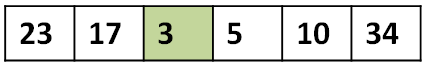
\includegraphics[width=0.3\textwidth]{pictures/selection1.png}
\caption{Unsorted Data Set}
\label{fig:selection1}
\end{figure}

3 is found as the smallest value.

\begin{figure}[H]
\centering
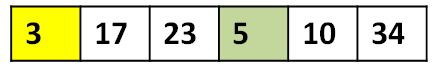
\includegraphics[width=0.3\textwidth]{pictures/selection2.png}
\label{fig:selection2}
\end{figure}

3 is placed at index 0 swapping with 23, 5 is found as the next smallest value.

\begin{figure}[H]
\centering
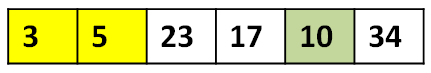
\includegraphics[width=0.3\textwidth]{pictures/selection3.png}
\label{fig:selection3}
\end{figure}

5 is placed at index 1, 10 is the next smallest value.

\begin{figure}[H]
\centering
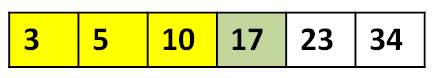
\includegraphics[width=0.3\textwidth]{pictures/selection4.png}
\label{fig:selection4}
\end{figure}

10 is placed at index 2. 17 is the next smallest value and it is already properly placed.

\begin{figure}[H]
\centering
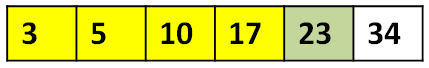
\includegraphics[width=0.3\textwidth]{pictures/selection5.png}
\label{fig:selection5}
\end{figure}

17 is placed at index 3. 23 is the next smallest value and it is already properly placed.

\begin{figure}[H]
\centering
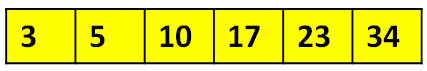
\includegraphics[width=0.3\textwidth]{pictures/selection6.png}
\label{fig:selection6}
\end{figure}

23 is placed at index 4. There is only one value left (34) which should be the largest value in the data set, no search is required for the last iteration.

\subsection{Pseudocode}

\begin{verbatim}
selectionSort(List):List
            1. Set lowestValue to index 0
            2. Search the range (lowestValue to max index) and find minimum value in the list
            3. Swap with value at location lowestValue
            4. Increment lowestValue to point to next index (shortening the search space)
            5. Repeat until list is sorted
            6. Return the List
\end{verbatim}


\section{Insertion Sort}
Insertion sort involves having a sorted sub-list within the list. The sub-list grows as the remaining list shrinks, until the entire list is the sorted sub-list. \newline

Insertion sort has a worst case complexity is O(n\textsuperscript{2}). Since it needs to shuffle the data set n times to make space for the next value. \newline

\begin{figure}[H]
\centering
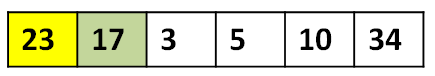
\includegraphics[width=0.3\textwidth]{pictures/insert1.png}
\caption{Unsorted Data Set}
\label{fig:insert1}
\end{figure}

The first element is already a sorted sub-list. 17 is to be placed before 23.

\begin{figure}[H]
\centering
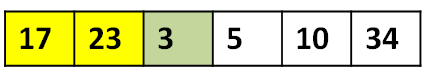
\includegraphics[width=0.3\textwidth]{pictures/insert2.png}
\label{fig:insert2}
\end{figure}

The sub-list is now 2 elements. 3 is to be placed before 17.

\begin{figure}[H]
\centering
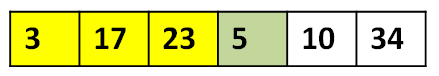
\includegraphics[width=0.3\textwidth]{pictures/insert3.png}
\label{fig:insert3}
\end{figure}

5 is to be placed after 3.

\begin{figure}[H]
\centering
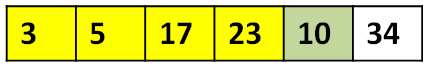
\includegraphics[width=0.3\textwidth]{pictures/insert4.png}
\label{fig:insert4}
\end{figure}

10 is to be placed after 10.

\begin{figure}[H]
\centering
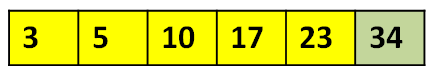
\includegraphics[width=0.3\textwidth]{pictures/insert5.png}
\label{fig:insert5}
\end{figure}

34 is to be placed after 23.

\begin{figure}[H]
\centering
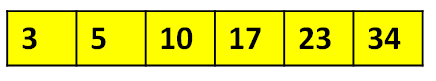
\includegraphics[width=0.3\textwidth]{pictures/insert6.png}
\label{fig:insert6}
\end{figure}

The sub-list now contains the whole list. The list is fully sorted.

\subsection{Pseudocode}

\begin{verbatim}
insertionSort(List):List
            1. If it is the first element, it is already sorted. Skip to step 6
            2. Increment to next element
            3. Compare with all elements in the sorted sub-list
            4. Shift all the elements in the sorted sub-list that is greater than the value 
                to be sorted, creating an empty element
            5. Insert the value
            6. Repeat until list is sorted
            7. Return the List
\end{verbatim}

\section{Shell Sort}

Shell sort uses insertion sort, but presorts sub-lists to reduce the number of shifts needed. The sub-lists are different from any type that we have looked at previously. The sub-lists are in a alternating pattern (1,2,3,1,2,3). This allows a single swap to replace n "shuffles", making it quite efficient. Next the number of intervals would be divided by 2 and done again. When the interval size is 3 or less, a final insertion sort will be done to finish the sort. 

Shell sort is very efficient with a worst case complexity of O(n).

\begin{figure}[H]
\centering
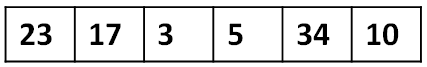
\includegraphics[width=0.3\textwidth]{pictures/shell1.png}
\label{fig:shell1}
\caption{Unsorted Data Set}
\end{figure}

\begin{figure}[H]
\centering
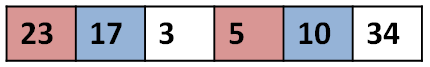
\includegraphics[width=0.3\textwidth]{pictures/shell2.png}
\label{fig:shell2}
\end{figure}

Here the sub-lists are at an interval of 3. This number is chosen based on the size of the data set.  

\begin{figure}[H]
\centering
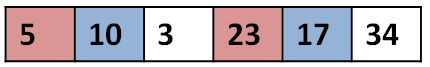
\includegraphics[width=0.3\textwidth]{pictures/shell3.png}
\label{fig:shell3}
\end{figure}

23 and 5 are compared and switched. 17 and 10 are compared and switched and 3 and 34 are compared and no switch was necessary. A total of 2 swaps were needed for the presort.

Since our interval was 3, the next step is to do an insertion sort (if our interval was greater, we would divide the interval by 2 and do this again).

\begin{figure}[H]
\centering
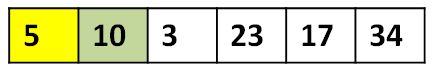
\includegraphics[width=0.3\textwidth]{pictures/shell4.png}
\label{fig:shell4}
\end{figure}

10 is inserted, no swaps were needed.

\begin{figure}[H]
\centering
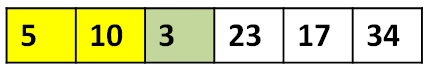
\includegraphics[width=0.3\textwidth]{pictures/shell5.png}
\label{fig:shell5}
\end{figure}

3 is inserted, 2 swaps are needed (10 and 3, then 5 and 3).

\begin{figure}[H]
\centering
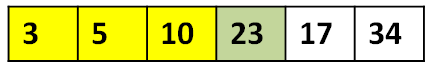
\includegraphics[width=0.3\textwidth]{pictures/shell6.png}
\label{fig:shell6}
\end{figure}

23 is inserted, no swaps were needed.

\begin{figure}[H]
\centering
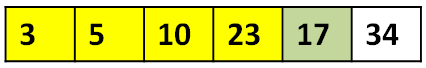
\includegraphics[width=0.3\textwidth]{pictures/shell7.png}
\label{fig:shell7}
\end{figure}

17 is inserted, 1 swap is needed.

\begin{figure}[H]
\centering
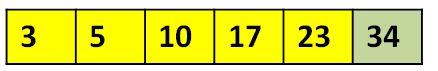
\includegraphics[width=0.3\textwidth]{pictures/shell8.png}
\label{fig:shell8}
\end{figure}

34 is inserted, no swaps were needed.

\begin{figure}[H]
\centering
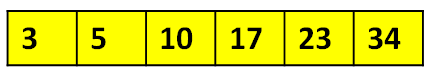
\includegraphics[width=0.3\textwidth]{pictures/shell9.png}
\label{fig:shell9}
\end{figure}

In total shell sort involved 5 swaps. In order to sort the same data set by just insertion sort 7 swaps are needed. As the data sets get larger, the need for shell sort increases.

\subsection{Pseudocode}

\begin{verbatim}
shellSort(List):List
            1. Initialize the interval of the sub-lists
            2. Divide the list into sub-lists
            3. Sort the sub-lists by swapping elements
            4. If the interval is greater than 3, divide it by 2 and go back to step 1. 
                Otherwise go to step 5.
            5. Combine sub-lists
            6. Use insertion sort on the whole list
            7. Return the List
\end{verbatim}


\section{Quick Sort}
Quick sort involves dividing the data set and sorting the segments recursively. A pivot is chosen to be the value at the highest index. Any values smaller than the pivot is placed on the left side of the "pivot wall" by swapping it with the value directly to the right of the wall. After a swap, the wall is incremented one place, to contain all smaller values.

Quick sort has a worst case complexity of O(n\textsuperscript{2}). More typically has a complexity of O(nlog(n)) when for each iteration the pivot value is at approximately the middle (value) of the data set.  

\begin{figure}[H]
\centering
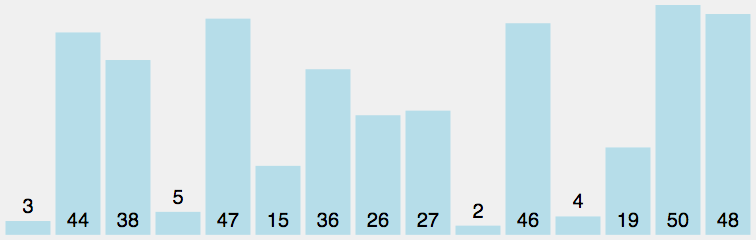
\includegraphics[width=0.3\textwidth]{pictures/quick1.png}
\label{fig:quick1}
\caption{Unsorted Data Set}
\end{figure}

\begin{figure}[H]
\centering
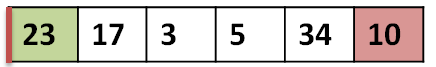
\includegraphics[width=0.3\textwidth]{pictures/quick2.png}
\label{fig:quick2}
\end{figure}

10 is at the highest index, so it is the pivot for this iteration. The wall starts before index 0 since there are no compared values yet. 23 is compared to 10, since it is greater no swap is needed.

\begin{figure}[H]
\centering
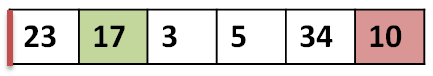
\includegraphics[width=0.3\textwidth]{pictures/quick3.png}
\label{fig:quick3}
\end{figure}

17 is compared to 10, no swap is needed.

\begin{figure}[H]
\centering
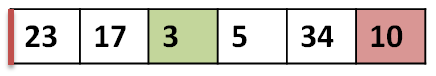
\includegraphics[width=0.3\textwidth]{pictures/quick4.png}
\label{fig:quick4}
\end{figure}

3 is compared to 10, a swap is needed. 3 will swap places with 23 (directly right of the wall). The wall will then increment to between index 0 and index 1. 

Note: swapping 23 does not affect the sort. It is still on the "greater than" side of the wall, and will be placed more precisely in recursive sorts.

\begin{figure}[H]
\centering
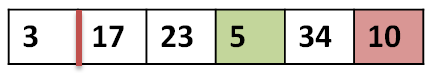
\includegraphics[width=0.3\textwidth]{pictures/quick5.png}
\label{fig:quick5}
\end{figure}

5 is compared to 10, a swap is needed. 5 swaps with 17 and the wall increments.

\begin{figure}[H]
\centering
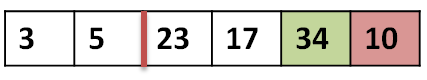
\includegraphics[width=0.3\textwidth]{pictures/quick6.png}
\label{fig:quick6}
\end{figure}

34 is compared to 10, no swap is needed. 
When the current index is equal to the pivot index (end of sort iteration), the pivot value is swapped with the value directly right of the wall. The wall \underline{does not} move. 

Note: If the wall is moved 10 would be the pivot for the recursive left sort, and everything is already known to be smaller. That is an infinite recursive loop waiting to happen.

\begin{figure}[H]
\centering
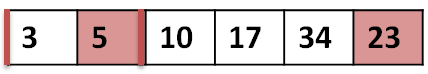
\includegraphics[width=0.3\textwidth]{pictures/quick7.png}
\label{fig:quick7}
\end{figure}

Next quick sort would be called to sort each of the sections. 5 would be the pivot for the left side with the wall at index 0 and 23 would be the pivot for the right side with the wall at the current position.

\subsection{Pseudocode}

\begin{verbatim}
quickSort(List, pivotIndex, startIndex):List
            1. Make the highest index value the pivot
            2. Partition the array using pivot value
            3. Quick sort left partition recursively
            4. Quick sort right partition recursively
            7. Return the List
\end{verbatim}

\section{Merge Sort}

Merge sort is another recursive function. It works be dividing the data set by 2 until it can no longer be divided, then recombining and sorting in the same order as it was divided. 

Merge sort is relatively robust sorting algorithm as it has a worst case complexity of O(nlog(n)). 

Note: Each colour represents a sub-list

\begin{figure}[H]
\centering
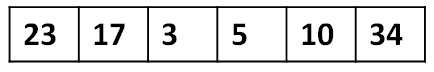
\includegraphics[width=0.3\textwidth]{pictures/merge1.png}
\label{fig:merge1}
\caption{Unsorted Data Set}
\end{figure}

\begin{figure}[H]
\centering
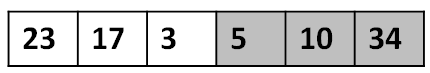
\includegraphics[width=0.3\textwidth]{pictures/merge2.png}
\label{fig:merge2}
\end{figure}

The data set is split into 2 sub-lists of length 3.

\begin{figure}[H]
\centering
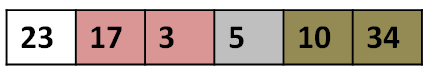
\includegraphics[width=0.3\textwidth]{pictures/merge3.png}
\label{fig:merge3}
\end{figure}

The sub-lists are split into 2 sub-lists (one of length len/2 and one of length (len/2 + len\%2))

\begin{figure}[H]
\centering
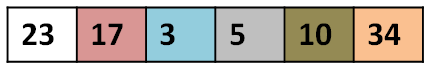
\includegraphics[width=0.3\textwidth]{pictures/merge4.png}
\label{fig:merge4}
\end{figure}

The sub-lists containing 23 and 5 can not be divided again. The remaining sub-lists are split again.

\begin{figure}[H]
\centering
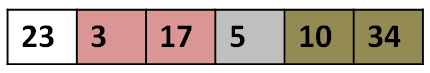
\includegraphics[width=0.3\textwidth]{pictures/merge5.png}
\label{fig:merge5}
\end{figure}

3 and 17 are sorted and recombined. 5 and 10 are recombined.

\begin{figure}[H]
\centering
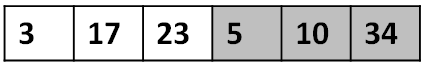
\includegraphics[width=0.3\textwidth]{pictures/merge6.png}
\label{fig:merge6}
\end{figure}

23 is sorted combined with 3 and 7. 5 is sorted and recombined with 10 and 34.

\begin{figure}[H]
\centering
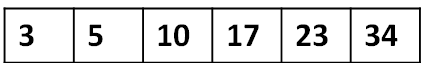
\includegraphics[width=0.3\textwidth]{pictures/merge7.png}
\label{fig:merge7}
\end{figure}

The 2 sub-lists are sorted and recombined. 

\subsection{Pseudocode}

\begin{verbatim}
mergeSort(List):List
            1. Check length of the list, if it is only one element it is already sorted, 
                skip to step 6
            2. Divide the list by 2 (one partition is len/2, the other would be (len/2 + len%2). 
                This accounts for numbers not divisible by 2) 
            3. Merge sort left partition recursively
            4. Merge sort right partition recursively
            5. Merge the smaller lists into new list in sorted order.
            6. Return the list
\end{verbatim}

